\documentclass[12pt,reqno,openany]{amsbook}
\usepackage{graphicx}
\usepackage{amsthm}
%\usepackage{mathpazo}
%\usepackage[scaled=0.9]{helvet}

\theoremstyle{plain}
\newtheorem{lem}{Lemma}[chapter]
\newtheorem{prop}{Proposition}[chapter]
\newtheorem{cor}{Corollary}[chapter]

\theoremstyle{definition}
\newtheorem{exmp}{Example}[chapter]

\usepackage{fancyhdr}
\pagestyle{fancy}
\fancyhf{}
\lhead{\tiny\thepage}
\chead{\tiny\rightmark}
\lfoot{\tiny\leftmark}
\rfoot{\tiny\texttt Version: 2.0}
\setlength{\footskip}{60pt}
\renewcommand{\headrulewidth}{0pt}

\newcommand{\newterm}[1]{\emph{#1}}


\title{Macroeconomics}
\author{Jyotirmoy Bhattacharya}
\address{Ambedkar University Delhi}
\email{jyotirmoy@jyotirmoy.net}
\date{\today}

\begin{document}
%\frontmatter
\maketitle
\tableofcontents
%\mainmatter
\chapter{Consumption: Certainty}
\section{Two-period case}
\subsection{Budget constraint}
Consider a consumer who lives for two periods, has an endowment of
$y_1$ and $y_2$ units of goods in the two periods respectively and can
borrow and lend any amount that they like at the real rate of interest
$r$. 

Suppose the consumer consumes $c_1$ in the
first period. Then she will have to take a loan of $c_1-y_1$ to
finance her consumption. (This number can be negative, in which case
the consumer is lending rather than borrowing.) In the next period the
consumer will therefore have to make loan repayments of
$(1+r)(c_1-y_1)$. Assume that the consumer does not want to make any
bequests and cannot die with any outstanding loans, consumption in the
second period must be,
\[c_2=y_2-(1+r)(c_1-y_1)\]
Simplifying and rearranging we have
\begin{equation}\label{eq:two-period-budget}
c_1+\frac{c_2}{1+r}=y_1+\frac{y_2}{1+r}
\end{equation}
This is the budget constraint faced by the consumer. We can interpret
this to mean that the present value of the consumer's consumption
stream must equal the present value of their incomes.

\subsection{Utility maximization}
Suppose the consumer maximises a quasiconcave utility function
$U(c_1,c_2)$ subject to this budget constraint. Then the consumer's
first-order conditions are
\begin{align}
U_1(c_1,c_2)&=\lambda\\
U_2(c_1,c_2)&=\lambda/(1+r)
\end{align}
where $\lambda$ is the Lagrange multiplier corresponding to the budget
constraint and $U_i(c_1,c_2)$ denotes the partial derivative $\partial
U/\partial c_i$. We have explicitly shown the dependence of the
partial derivatives on the value of consumption in both periods. These
first-order conditions along with the budget
constraint~\eqref{eq:two-period-budget} together determines the value
of $c_1$, $c_2$ and~$\lambda$.
\subsection{Comparative statics}
Assuming that consumption in both periods is a normal good, an
increase in either $y_1$ or $y_2$ increases both $c_1$ and $c_2$.

The effects of a change in $r$ are ambiguous. An increase in $r$ makes
consumption in period~$2$ relatively cheap compared to consumption in
period~$1$. Therefore the substitution effect causes $c_1$ to decrease
and $c_2$ to increase. It is traditional to decompose the income
effect into two parts. First, an increase in $r$ reduces the present
value of the consumer's endowments and hence decreases his real
income. Second, an increase in $r$, by making the consumption in
period~$2$ cheaper increases his real income.\footnote{
For more about the Slutsky equation in the case of a consumer with
fixed endowments of goods see section~9.1 in Varian's
\emph{Microeconomic Analysis}, 3rd ed.} The sign of the
resultant of these two effects on consumption depends on whether the
consumer is a net lender in period~1 and a net borrower in period~2 or
vice-versa. In case the consumer is a net lender in period~1 and a net
borrower in period~2 the net income effect is positive. Assuming the
consumption in both periods in a normal good, this means that the
substitution effect and the income effect act in opposite directions
on $c_1$ in this case leading to an ambiguous effect.

\section{Many periods}
Assume that rather than just living for two periods the consumer lives
for $T+1$ periods. Further assume that the real rate of interest takes a
constant value $r$ over the consumer's lifetime. For convenience we
define $\delta=1/(1+r)$. It is also convenient to start time from
period~0 rather than period~1.

\subsection{Budget constraint}
Arguing as before, the consumer's budget constraint is
\begin{equation}\label{eq:many-period-budget}
\sum_{i=0}^T \delta^i c_i = \sum_{i=0}^T \delta^i y_i
\end{equation}

\subsection{Utility function}
We could proceed as before by assuming a utility function
$U(c_0,\ldots,c_T)$ and deriving the first order conditions. However,
because the marginal utility in each period depends on consumption in
all periods it is hard to draw any sharp conclusions at this level of
generality. Therefore we need to impose some restrictions on the form
of the utility functions.

Suppose, for example we assume that the utility function is additively
separable, i.e.

\begin{equation}\label{eq:utility-addsep}
U(c_0,\ldots,c_T)=v_0(c_0)+v_1(c_1)+\cdots+v_T(c_T)
\end{equation}

Then the first-order conditions take the form

\begin{equation}\label{eq:foc-additively-separable}
v_i'(c_i) = \delta^i \lambda \qquad i=0,\ldots,T
\end{equation}
where, as before, $\lambda$ is the Lagrange multiplier corresponding
to the budget constraint.

Sometimes we want to restrict the consumers preferences even further,
by assuming that the different $v_i$ differ from each other by only a
geometric discounting factor.

\begin{equation}\label{eq:utility-geometric}
U(c_0,\ldots,c_T)=\sum_{i=0}^T \beta^i u(c_i)
\end{equation}
where $\beta$ is a constant, referred to as the subjective rate of
discount, such that $0<\beta<1$.  

In this case the first-order conditions take the particularly simple
form
\begin{equation}\label{eq:foc-stationary}
u'(c_i)=\left(\frac{\delta}{\beta}\right)^i \lambda \qquad i=0,\ldots,T
\end{equation}

In case $\delta=\beta$, this implies that $u'(c_i)$ is the same for
all $i$, which, assuming that $u'(\cdot)$ is a strictly decreasing
function, means that $c_i$ is constant for all $i$. The present
period's income does not influence the present period's consumption at
all. Consumption is determined solely by lifetime resources as given
by~\eqref{eq:many-period-budget}.

The case $\delta \neq \beta$ is also instructive. Suppose
$\delta>\beta$. In this case it follows from~\eqref{eq:foc-stationary}
that consumption decreases over time. Formally, this is because if
$\delta>\beta$ then by~\eqref{eq:foc-stationary} $u'(c_i)$ increases
over time, and since $u'(c)$ is a decreasing function of consumption,
this implies that $c$ decreases over time. 

The economic logic behind this result is that $\delta$ is the number of
units of consumption we have to give up at present in order to
purchase one more unit of consumption next period, whereas $\beta$ is
the number of units of marginal utility we are willing to give up at
present in order to have one more unit of marginal utility in the next
period. Suppose we start with the same consumption $c$ in this period and
the next. If we reduce consumption in the next period by a small
amount $\Delta c$ then at the prevailing market prices we can
increase present consumption by $\delta\Delta c$. The increase in
utility from the increase in present consumption is approximately
$u'(c)(\delta\Delta c)$.\footnote{We are using Taylor's theorem:
  $u(c+\delta\Delta c)-u(c) \approx u'(c)(\delta\Delta c)$} The decrease in utility from the reduction in
next period's consumption is approximately $\beta u'(c)(\Delta c)$. The
net change in utility would be $(\delta-\beta)u'(c)(\Delta c)$ which
is positive when $\delta>\beta$. Thus it is beneficial to increase present consumption and
reduce future consumption if we are starting from a position of
equality. Indeed, it will be optimal to increase consumption in the
present period (say period $i$) and decrease consumption in the next
period (period $i+1$) till the following equality between the MRS and
the price ratio is satisfied,
\[\frac{u'(c_{i+1})}{u'(c_i)}=\frac{\delta}{\beta}\]

If $\delta/\beta$ is close to $1$ then $c_{i+1}$ is close to $c_i$ and
we can use Taylor's Theorem from calculus to the above equation to the
above equation to get a useful approximation.
\begin{align*}
\frac{u'(c_{i+1})}{u'(c_i)}&=\frac{\delta}{\beta}\\
\frac{u'(c_{i+1})-u'(c_i)}{u'(c_i)}&=\frac{\delta}{\beta}-1\\
\intertext{Applying Taylor's Theorem}
\frac{u''(c_i)(c_{i+1}-c_i)}{u'(c_i)}&\approx\frac{\delta}{\beta}-1\\
\intertext{Defining $\Delta c=c_{i+1}-c_i$, and dropping the subscript
$i$,}
\left(\frac{u''(c)c}{u'(c)}\right)\left(\frac{\Delta
    c}{c}\right)
&\approx\frac{\delta}{\beta}-1\\
\intertext{The quantity $\sigma=-u''(c)c/u'(c)$ is known as the
  \emph{intertemporal elasticity of substitution} and captures the
  sensitivity of marginal utility of changes in consumption. It is positive since marginal utility
  decreases with consumption.}
\left(\frac{\Delta
    c}{c}\right)&\approx
\frac{1}{\sigma}\left(1-\frac{\delta}{\beta}\right)
\end{align*}
The formula confirms our earlier reasoning that consumption decreases
over time if $\delta>\beta$. Moreover, it shows that the sensitivity
of the growth of consumption on the rate of return depends inversely
on the intertemporal elasticity of substitution. The reason for this
is that the more elastic is marginal utility to consumption, the smaller
is the deviation in consumption from a constant path that is required
the equate the ratio of marginal utilities in consecutive time periods
to $\delta/\beta$.
\subsection{Exogenous variables}
It is possible to unify~\eqref{eq:utility-addsep}
and~\eqref{eq:utility-geometric} by writing
\[v_i(c_i)=\beta^i u(c_i,\xi_i)\]
where $\xi_i$ is an exogenous variable such a the consumer's age or
the number of members in the household. In this case the first-order
conditions become
\[u'(c_i,\xi_i)=\left(\frac{\delta}{\beta}\right)^i \lambda \qquad
i=0,\ldots,T\]
Knowing how $\xi$ affects the marginal utility would
now let us make some predictions regarding the path of consumption.

\subsection{Comparative statics}
Assuming that consumption in every period is a normal good, an
increase in $y_i$ increases every $c_i$.

The effect of an increase in $r$, or equivalently, a decrease in
$\delta$ remains ambiguous because of the same income and substitution
effects as discussed earlier. But for the utility function given
by~\eqref{eq:utility-geometric}, we can say a little
more. From~\eqref{eq:foc-stationary} we can see that a decrease in
$\delta$ means that the \emph{growth rate} of consumption speeds
up. Remember that even in this case we do not have any information
regarding the \emph{level} of consumption in any period since the
level would depend on $\lambda$ which in turn depends on $\delta$.
\chapter{The Envelope Theorem}
\section{Parametrised optimisation problems}
Let's think of unconstrained problems first. Every optimisation
problem has an objective function. It is the function that we are
trying to maximise or minimise (henceforth maximise). Some of the variables entering the
objective function are \emph{choice variables}, variables whose values
we are free to choose in order to maximise the objective function. But
all the variables entering into the objective function need not be
choice variables. The value of the objective function may also depend
on the value of other variables which we are not free to choose. We
call these the \emph{parameters} of the optimisation problem. 

\begin{exmp}\label{exmp:opti:profit}
Consider the short-term profit
maximising problem of a firm that produces according
to the production function
\[y=f(L,K)=L^{1/2}K^{1/2}\]
In the short-run the capital stock of the firm is fixed at some value
$\bar K$ and the firm can only choose the labour input $L$. If the
firms buys labour and capital in perfectly competitive labour market at prices
$w$ and $r$ respectively and sells its output in a perfectly competitive market at the
price $p$ then its profits are:
\[\pi(L,\bar K)=py-wL-r\bar K=pL^{1/2}{\bar K}^{1/2}-wL-r\bar K\]

For the short-run profit maximising problem $\pi(L,\bar K)$ is the
objective function, with $L$ as a choice variable and $\bar K$ as a
parameter.\footnote{In fact $p$, $r$ and $w$ are also parameters in
  the profit function. But we shall ignore this fact for now since we
  will not be looking at the effects of changes in these variables.}

Denoting the optimal amount of labour input by $L^*$, the first-order condition for profit maximisation is,
\begin{align*}
\frac{\partial \pi}{\partial L}&=0\\
\frac{1}{2}p{L^*}^{-1/2}{\bar K}^{1/2}-w&=0\\
L^*&={\bar K}(p/2w)^2
\end{align*}

You should check that $\pi(L,\bar K)$ is a concave function of $L$ and
therefore the first-order condition is sufficient to give us a global
maximum. The profit earned by the firm at the optimal point is,
\begin{align*}
\pi^*&=\pi(L^*,\bar K)\\
&=p[{\bar K}^{1/2}(p/2w)]{\bar K}^{1/2}-w[{\bar K}(p/2w)^2]-r\bar K\\
&={\bar K}(p^2/2w)-{\bar K}(p^2/4w)-r\bar K\\
&={\bar K}(p^2/4w)-r\bar K
\end{align*}

We see that both the amount of labour input chosen by the firm and the
maximum profit it earns are functions of the value of the parameter
$\bar K$. The function mapping the parameter values to the maximum (or
minimum) value of the objective function is called the \emph{value
  function}. In this case, denoting the value function by $V(\cdot)$
we have,
\[V(\bar K)=\pi^*={\bar K}(p^2/4w)-r\bar K\]
\qed
\end{exmp}

\section{The envelope theorem}
How does the optimal value change when we change the parameters? In
our example since we have an explicit formula for the value function
we can calculate its value directly
\[V'(\bar K) =(p^2/4w)-r\bar K\]

Even when we do not have an explicit formula for the value function,
there is an interesting relationship between the partial derivatives
of the objective function and the partial derivatives of the value
function.

Consider the general problem of maximising the objective function
\[\phi(x_1,\ldots,x_n;c_1,\cdots,c_m)\]
where the $x_i$ are choice variables and $c_i$ are parameters.

The first order conditions for the problem are,
\begin{equation}\label{eq:opti:foc}
\frac{\partial \phi}{\partial
  x_i}(x_1,\ldots,x_n;c_1,\ldots,c_m)=0\qquad i=1,\cdots,n
\end{equation}

Just as in the example, the optimal values of the choice variables,
denoted by $x_i^*$, will be functions of the parameters
$c_1,\ldots,c_m$. The value function will be given by
\[V(c_1,\ldots,c_m)=\phi(x_1^*,\ldots,x_n^*;c_1,\ldots,c_m)\]

Suppose we want to calculate the partial derivative of the value
function with respect to one of the parameters, say $c_j$. In doing so
we have to take into account the fact that the optimal value of each
of the choice variables would also be a function of $c_i$. So we use the
chain rule,
\[\frac{\partial V}{\partial c_j}=
\frac{\partial \phi}{\partial x_1}\frac{\partial x_1^*}{\partial c_j}
+\cdots
+\frac{\partial \phi}{\partial x_n}\frac{\partial x_n^*}{\partial c_j}
+\frac{\partial \phi}{\partial c_j}
\]

However, from~\eqref{eq:opti:foc}, we know that $\partial
\phi/\partial x_i$ is $0$ for all $i$ when the partial derivatives are
evaluated at the optimal values. So we have,
\begin{equation}\label{eq:opti:envelope}
\frac{\partial V}{\partial c_j}=\frac{\partial \phi}{\partial c_j}
\end{equation}

This remarkably is the same result that we would have got if we had
treated each of the $x_i^*$ as a constant. But that would not have
been justified since the choice variables do vary when parameters are
varied. That is, $\partial x_i^*/\partial c_j$ is generally not zero.
It is just that when we are starting from an optimal point then the
marginal impact on this variation on the objective function (i.e.,
$\partial \phi/\partial x_i$ is zero and therefore we can ignore the
changes in the choice variables.

Equation~\eqref{eq:opti:envelope} is known as the ``Envelope
Theorem''.

\section{Geometric Interpretation}
\begin{figure}
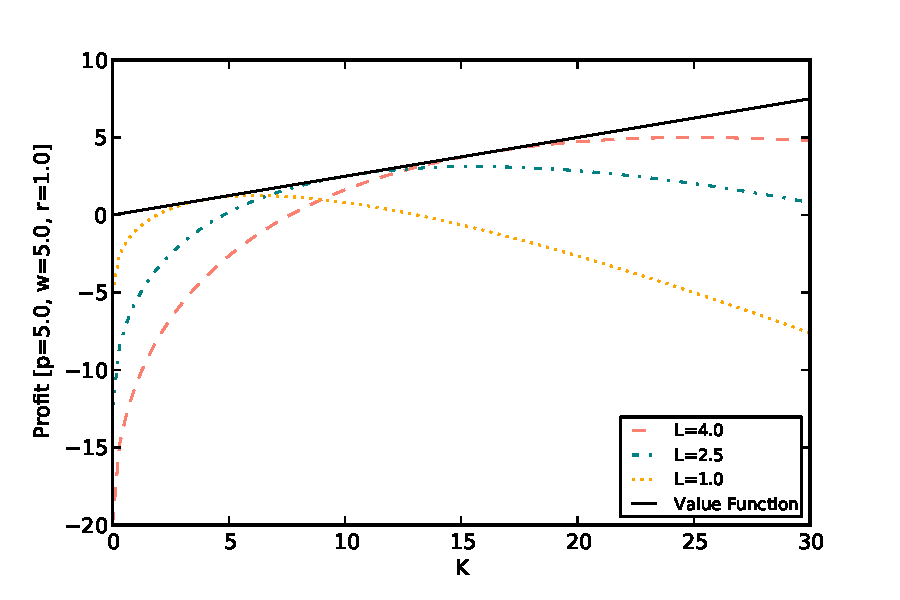
\includegraphics[width=0.9\textwidth]{envelope.pdf}
\caption{The Envelope Theorem}\label{fig:opti:envelope}
\end{figure}
Figure~\ref{fig:opti:envelope} illustrates the envelope theorem in the
case of Example~\ref{exmp:opti:profit}. Each of the coloured curves
shows the level of profit for a given level of $L$ and for different
values of $K$. Let's call them ``profit curves''.\footnote{This is not
  standard terminology and you must
remember that these curves are not graphs of the full profit function since we
are holding $L$ constant on each of them.} We have drawn only three of
these curves but you should imagine there to be one curve for each
possible value of $L$. Now, since our purpose is to maximise profit
for a given value of $K$, we move along a vertical line for our
particular value of $K$ and choose that $L$ whose profit curve is the
highest at that value of $K$.

Thus, for example, at $K=4.0$ we would choose $L=4.0$ whereas at
$K=10.0$ we would choose $L=2.5$.

The value of the highest profit curve for a given $K$ gives us the
highest profit we can obtain when $K$ takes on that value. But that is
precisely the definition of the value function. Therefore the graph of
the value function touches the highest of the profit curves at each
$K$. Or, in other words, the graph of the value function (the black
line in the figure)  must be the upper
envelope of the graphs of the profit functions for given values of
$L$. 

Since the value function is the upper envelope of the profit curves,
no profit curve can ever cross it. But at each value of $K$ one of the
profit curves, corresponding to the optimal $L$, touches it. The only
way two graphs can touch without crossing is if they are tangent to
each other. The slope of the graph of the value function is $\partial
V/\partial K$ whereas the slope of the profit curves is $\partial
\pi/\partial K$. Tangency of the two graphs implies that these slopes
should be equal, which is precisely what our the envelope theorem in
eq.~\eqref{eq:opti:envelope} also says when applied to this example.

Now you know what the envelope theorem is called by that name.

\section{Constrained Optimisation}
So far we have discussed unconstrained problems. There is also a
version of the envelope theorem for constrained optimisation problems.
Suppose our problem is to maximise
\begin{equation*}
\phi(x_1,\ldots,x_n;c_1,\ldots,c_m)\\
\end{equation*}
subject to the constraint
\begin{equation}\label{eq:opti:constraint}
h(x_1,\ldots,x_n;c_,\ldots,c_m)=0
\end{equation}
Here we have allowed both the objective function and the constraint to
depend on a set of parameters.

The first-order condition for this problem is
\begin{equation}\label{eq:opti:cfoc}
\frac{\partial \phi}{\partial x_i}
=\lambda \frac{\partial h}{\partial  x_i}
\qquad i=1,\ldots n
\end{equation}
where $\lambda$ is a Lagrange multiplier.

As before, if the problem has a solution the optimal values of the
choice variables, the $x_i^*$, will be functions of the parameters of
the problem. Also as before, we can define the value function as
\[V(c_1,\ldots,c_m)=\phi(x_1^*,\ldots,x_n^*;c_1,\ldots,c_m)\]

Differentiating the value function with respect to $c_j$ gives us,
\begin{equation}\label{eq:opti:value-chain}
\frac{\partial V}{\partial c_j}=
\frac{\partial \phi}{\partial x_1}\frac{\partial x^*_1}{\partial c_j}
+\cdots
+\frac{\partial \phi}{\partial x_n}\frac{\partial x^*_n}{\partial c_j}
+\frac{\partial \phi}{\partial c_j}
\end{equation}

To simplify this we need to digress a bit. The optimal values of the
choice variables must satisfy the
constraint~\eqref{eq:opti:constraint} for all values of the parameters, so we have
\[h(x_1^*,\ldots,x_n^*;c_,\ldots,c_m)=0.\]
Differentiating this with respect to
$c_j$ we get
\[\frac{\partial h}{\partial x_1}\frac{\partial x^*_1}{\partial c_j}
+\cdots
+\frac{\partial h}{\partial x_n}\frac{\partial x^*_n}{\partial c_j}
+\frac{\partial h}{\partial c_j}=0\]
Substituting the first-order conditions~\eqref{eq:opti:cfoc} we have,
\[\frac{1}{\lambda}\frac{\partial \phi}{\partial x_1}\frac{\partial x^*_1}{\partial c_j}
+\cdots
+\frac{1}{\lambda}\frac{\partial \phi}{\partial x_n}\frac{\partial x^*_n}{\partial c_j}
+\frac{\partial h}{\partial c_j}=0\]
or,
\[\frac{\partial \phi}{\partial x_1}\frac{\partial x^*_1}{\partial c_j}
+\cdots
+\frac{\partial \phi}{\partial x_n}\frac{\partial x^*_n}{\partial c_j}
=-\lambda\frac{\partial h}{\partial c_j}\]

Now this can be substituted in~\eqref{eq:opti:value-chain} to give us
\begin{equation}\label{eq:opti:cenvelope}
\frac{\partial V}{\partial c_j}=
-\lambda\frac{\partial h}{\partial  c_j}
+\frac{\partial \phi}{\partial c_j}
\end{equation}

Equation~\eqref{eq:opti:cenvelope} is the envelope theorem for the
constrained case. It is similar to the unconstrained envelope theorem
in that the change in the choice variables as a result of the change
in the parameters drops out of the calculation. It differs  in that the
change in the value function as a result of a change in a parameter
depends not just on the direct change in the objective function
($\partial \phi/\partial c_j$) but also the
change in constraint set ($\partial h/\partial c_j$). The Lagrange multiplier
$\lambda$ can be interpreted as a sensitivity factor, indicating the
extent to which a given change in the constraint set translates into a
change in the value function.

\begin{exmp}
Consider the problem of maximising the utility function $U(x_1,x_2)$
subject to the budget constraint $p_1x_1+p_2x_2=M$. Treating $x_1$ and
$x_2$ as choice variables and $p_1$, $p_2$ and $M$ as parameters, we
have the objective function
\[\phi(x_1,x_2;p_1,p_2,M) = U(x_1,x_2)\]
and the constraint function
\[h(x_1,x_2;p_1,p_2,M)=p_1x_1+p_2x_2-M\]

In this case the value function $V(p_1,p_2,M)$ is important enough to
be given a name. It is called the \emph{indirect utility function}.

If the value of the Lagrange multiplier at a the optimal bundle is
$\lambda$, then the envelope theorem~\eqref{eq:opti:cenvelope} tells
us that,
\begin{align*}
\frac{\partial V}{\partial M}&=
-\lambda\frac{\partial h}{\partial  M}
+\frac{\partial \phi}{\partial M}\\
&=-\lambda \cdot -1+0\\
&=\lambda
\end{align*}

This gives us an economic interpretation of the Lagrange multiplier.
It measures the amount by which the maximum attainable utility
increases per unit increase in income. In looser phrasing, it is the
``marginal utility of income''.

\qed
\end{exmp}

\chapter{Dynamic programming}
\section{The setup}
In a dynamic optimisation problem, our goal is to find a \emph{path}
of the choice variable which maximises the value of an objective
function defined over the entire path of the choice variable. Often,
there are constraints on what paths can be chosen. For example, in the
consumption-saving problem we choose a path of consumption which
maximises the lifetime utility function subject to a budget
constraint.

The dynamic programming approach to solving dynamic optimisation
problems  turns this single large optimization problem into a
sequence of simple optimization problems. At each point of time we try
to find the best action at that particular point of time. But since
this is a dynamic problem after all, this search for the best actions
at a particular point of time has to be done with an eye on both the
past and the future. Past events and actions\footnote{We want to make
  a distinction between \emph{events} which are outside of our control
  and \emph{actions} which are things we choose. This distinction
  becomes important when we are dealing with uncertainty.} determine what choices can be made now. By the
same token, the action that we take now will change the options
available to us the in future. The value of the objective function
that will be achieved will in general depend on the entire path of
past, present and future actions and not just the action in any period in
isolation.

In the dynamic programming framework this linkage between the past and
the future is captured by the notion of the \emph{state}. Intuitively,
we can think of the state at any given point of time as a description
of all the \emph{relevant} information about the actions and events
that have happened until that point. The state should contain all the
information that is required from the decision-maker's history to
determine the set of available actions at future points of time and to
evaluate the contribution made by future actions to the objective
function.

The notion that knowing the state at a point of time is enough to know
what actions are possible in the future is captured by the following definitions:
\begin{description}
\item[Set of states ($S_t$)] this is the set of possible states the
  decision-maker can be in time $t$. There is one such set for each time
  period $t$. The elements of these sets, i.e. the possible states,
  are assumed to be vectors with real-number elements. Elements of
  this set are denoted by $s_t$.
\item[Set of actions ($A_t$)] this is the set of possible actions that
  can be taken at time $t$. Elements of this set are denoted by
  $a_t$. As we shall see next, all possible actions cannot be taken at
  all possible states.
\item[Constraint correspondence $f_t(s_t) \subset A_t$] this tells
  us the subset of actions that are available in a particular
  state. This is  not a function but a correspondence (i.e.~a
  set-valued function) since for
  each element of $S_t$ it gives us a subset and not just a single
  element of $A_t$. 
\item[Transition function $\Gamma_t(s_t,a_t) \in S_{t+1}$] This tells us
  our state in period $t+1$ if we take the action $a_t$ in state $s_t$
  in period $t$.
\end{description}

With these definitions in hand we can define the set of \emph{feasible
  plans} when starting with $s_t$ at time $t$, denoted by
$\Phi_t(s_t)$, as the set of sequences of actions $(a_t,\ldots,a_T)$
such that
\[a_i \in f_i(s_i) \quad \text{for $i=t,\ldots,T$}\]
and
\[s_{i+1} = \Gamma_i(s_i,a_i) \quad \text{for $i=t,\ldots,T-1$}\]
The first condition says that the action taken on each date is a
feasible action given the state. The second condition says that the
state at each date is derived from the state and action taken in the
previous date, with the state at time $t$ as given.

The set of feasible plans tells us about the constraints faced in our
optimisation problem. What about the objective function? We assume
that the objective function can be written in an additively separable
form
\[U_t(a_t,s_t,\ldots,a_T,s_T)=\sum_{i=t}^T v_i(a_i,s_i)\]
where $v_t(a_t,s_t)$ is the \emph{per-period payoff function} that
gives the contribution of action $a_t$ in state $s_t$ at time $t$ to
the overall objective. Being able to write the objective function in
an additively separable form is essential for us to be able to use
dynamic programming.\footnote{We are cheating a bit here. The
  assumption of additive separability can be relaxed to what is called
  `recursiveness' while still allowing the use of dynamic
  programming.}

In writing the above objective function we have also
assumed that there is a finite time period $T$ at which our
optimisation problem comes to an end. This assumption of what is known
as a finite horizon is made just to simplify the mathematics. Dynamic
programming problems with an infinite horizon are routinely used in
economic modelling.

The solution to the dynamic programming problem is expressed in terms
of two functions:
\begin{description}
\item[Policy function $g_t(s_t) \in f_t(s_t)$] The policy function
  tells us the best action to take in each possible state at time $t$
  among all the available actions. In general it is possible that
  there be two equally good actions at a particular state, in which
  case the policy function would have to be replaced by the policy
  correspondence.
\item[Value function $V_t(s_t) \in \mathbb{R}$] The value function
  denotes the maximum attainable value of the objective function when
  starting at time $t$ from state $s_t$. That is,
  \begin{equation*}
    \begin{split}
      V_t(s_t) &= \max_{(a_t,\ldots,a_T) \in \Phi_t(s_t)}\,
      U_t(a_t,s_t,\ldots,a_T,s_T)\\
      &=\max_{(a_t,\ldots,a_T) \in
        \Phi_t(s_t)}\,[v_t(a_t,s_t)+\cdots+v_T(a_T,s_T)]
      \end{split}
    \end{equation*}
\end{description}

In applications of dynamic programming we generally want to know the
optimal path starting at a specific point of time (taken to be $t=0$
here) and from a particular state at that point of time (say $\bar
s_0$). But we have defined the policy and value functions for all
points of time and for each possible state at each of the time
periods. Thus it would seem that we have multiplied our work manyfold
beyond what is necessary for our original problem. But as we shall see
below, being willing to contemplate the policy and value functions for
all possible time periods and states often actually simplifies the
task of solving the original problem.

\section{Bellman's Principle of Optimality} 
Suppose I am starting at some time $t<T$ from some particular state $s_t$ and
trying to find the best actions from time $t$ to $T$, where `best'
means the choices of actions and consequent states which maximise 
\[U_t(a_t,s_t,\ldots,a_T,s_T)=\sum_{i=t}^T v_i(a_i,s_i).\] 
Because of the additive nature of the lifetime utility function we can
rewrite the above equation as
\[U_t(a_t,s_t,\ldots,a_T,s_T)=v_t(a_t,s_t)+U_{t+1}(a_{t+1},s_{t+1},\ldots,a_T,s_T)\]
If we divide the plan (path of actions and corresponding states) from
time $t$ to time $T$ into a ``head'' consisting of the action in
period $t$ and a ``tail'' consisting of actions in period $t+1$ to $T$
then the above equation says that the lifetime utility of the plan
starting at period $t$ is the sum of the per-period payoff at time $t$
(the value of the ``head'') and the lifetime utility of the remaining
part of the plan from period $t+1$ onwards (the value of the
``tail'').

How do we find the plan which maximises $U_t$? Suppose we choose the
action $\hat a_t$ in period $t$. This will lead us to the state $\hat
s_{t+1}=\Gamma_t(s_t,\hat a_t)$ in the next period. Now we have to
pick a plan from period $t+1$ onward. Now $U_t=v_t(\hat
a_t,s_t)+U_{t+1}$ and $v_t(\hat a_t,s_t)$ is already fixed by our
choice of action $\hat a_t$ in period $t$. Therefore in choosing our
plan from period $t+1$ onward the best we can do is to pick a plan
that maximises $U_{t+1}$. This optimal plan for the ``tail'' yields
the value of $U_{t+1}$ equal to $V_{t+1}(\hat s_{t+1})$. Thus we can
evaluate each choice of action $\hat a_t$ in the ``head'' by looking
at 
\[\tilde U_t=v_t(\hat a_t,s_t)+V_{t+1}(\hat s_{t+1}),\quad 
\text {where $\hat s_{t+1}=\Gamma(s_t,\hat a_t)$}\]
We have put a tilde over $U_t$ to remind ourselves that now we are not
considering arbitrary plans starting at $t$ but only plans where the
``tail'' component is optimal given the state $\hat s_{t+1}$ at which
we find ourselves in the beginning of period $t+1$. 

The optimal plan from period $t$ involves choosing $\hat a_t$ which
maximises the expression above. Since the value function gives the
value of the objective function $U_t$ for the optimal plan, it is
therefore the case that,
\begin{equation}\label{dp:the-bellman}
V_t(s_t)=\max_{\hat a_t \in f_t(s_t)}\,[v_t(\hat
  a_t,s_t)+V_{t+1}(\Gamma(s_t,\hat a_t))], \quad \text{for $t<T$}
\end{equation}

Equation~\eqref{dp:the-bellman} above which relates the value function
at consecutive time periods is known as \emph{Bellman's
  Equation}. The argument above, which shows that the value function
must satisfy Bellman's equation is known as \emph{Bellman's Principle
  of Optimality}.\footnote{To be complete, Bellman's principle of
  optimality also deals with the converse: that a function which
  satisfies Bellman's equation plus some other technical conditions
  must be the value function. This converse is not important in our
  current finite horizon setting.}

Intuitively Bellman's equation tells us that we can evaluate each present
action by adding its contribution $v_t(\hat a_t,s_t)$ to the objective
in the present period and the value $V_{t+1}(\hat s_{t+1})$ of the
state in which
it leaves us in the next period. Provided we know the function
$V_{t+1}$ for all possible states in the next period we can choose the
best action in the current period by choosing $\hat a_t$ to maximise
this sum. Thus we have turned the big optimisation problem of choosing
an entire sequence of actions from time $0$ to time $T$ into a
sequence of simple optimisation problems, one for each time period
$t$, in each of which we choose a single action $\hat a_t$.

But there seems to be a chicken-and-egg problem: we cannot use
Bellman's equation without knowing $V_{t+1}$ for each $t$ and how do
we know $V_{t+1}$ if we have not solved the optimisation problem
already? Here our finite horizon assumption makes life particularly
simple for us. 

Since period $T$ is the last period, our objective function in that
period is
\[U_T(a_T,s_T)=v_T(a_T,s_T)\]
and the value function is simply given by
\[V_T(s_T)=\max_{a_T \in f_T(s_T)}\, v_T(a_T,s_T)\] We can solve this
maximisation problem and calculate $V_T$ since $v_T(\cdot,\cdot)$ is a
known function.

Now consider Bellman's equation for period $T-1$:
\[V_{T-1}(s_{T-1})=\max_{\hat a_{T-1} \in f_t(s_{T-1})}\,
[v_{T-1}( \hat a_{T-1},s_{T-1})+V_T(\Gamma(s_{T-1},\hat a_{T-1}))]\]

As we have calculated $V_T(\cdot)$ in the previous step, all the
functions in the maximisation problem are known and we can solve the
problem to calculate $V_{T-1}$. With this in hand we can solve
Bellman's equation for period $T-2$. We keep going backward one period
at a time until we have calculated the value function for all periods
until period $0$. At each step the value of $\hat a_t$, as a function
of $s_t$, which solves the maximisation problem gives us the policy
function. So by the end of our process we also have the policy
function for each time period. 

Now if we are given a starting state $\bar s_0$ in period $0$ we can
use the calculated policy function for period $0$ to find the best
action $a_0$ in period 0. We know from the transition function that we
will end up in state $s_1=\Gamma(\bar s_0,a_0)$ in the next
period. The policy function for period~$1$ tells us the best action
$a_1$ to take in that period. We again use the transition function to
tell us the next state $s_2=\Gamma(s_1,a_1)$. And so on until we have
traced out the optimal plan to time $T$. Our optimisation problem is
solved! 

The way we have calculated the value function backwards from a
known final time period is sometimes called ``backward induction''.

\section{Example: consumption-savings with log utility}
Suppose that the consumer maximises
\[\sum_{i=0}^T \log(c_i)\]
subject to
\[\sum_{i=0}^T c_i/R^i=w_0\]

Can we solve this maximisation problem using dynamic programming? The
action variable in this case must be $c_i$ since it is the variable
being chosen by the decision maker. The
objective function is already in an additively separable form with a
per-period payoff $\log(c_i)$. But what is the state?

Since the per-period payoff depends only on the action variable $c_i$
we do not need any notion of state to evaluate payoffs. But the choice
of a consumption in each period does affect future periods through the
budget. The more we consume today, the less purchasing power we have
to consume tomorrow. We can capture this by rearranging the budget
slightly to read,
\[\sum_{i=1}^T c_i/R^i = w_0-c_0\]
Multiplying throughout by $R$ we have
\[\sum_{i=1}^T c_i/R^{(i-1)} = R(w_0-c_0)\]
Which shows us that the path of consumption from time~1 onwards
follows a budget constraint of the same form as the period~0 budget
constraint provided we take
\[w_1=R(w_0-c_0)\]
This suggests to us that we can take the wealth at the beginning of
period~$t$ as our state with the transition function,
\[w_{t+1}=R(w_t-c_t),\quad \text{for $t=0,\ldots,T$}\]
and the constraint function
\[c_T = w_T\]
The constraint captures the fact that there can be no outstanding debt
in the last period and a consumer who has monotonic preferences would
not leave any wealth unused in the last period. There is no constraint
on consumption in periods other that $T$.\footnote{We could have
  imposed a non-negativity constraint but we leave it out for simplicity}.

You can check that we have formulated the problem right by eliminating
$w_1,\ldots,w_T$ in the transition functions and constraints above to
recover our original budget constraint. 

Now we can use backward induction to calculate the value function and
policy function for all time periods. Denoting the policy function by $g(\cdot)$ and the value
function in period $t$ by $V_t(\cdot)$, we have,
\begin{equation}\label{eq:dplog-T}
g_T(w) = w,\qquad V_T(w_T) = \log(g_T(w))=\log(w)
\end{equation}

Now consider period $T-1$. Bellman's principle of optimality tells us,
\begin{equation}\label{eq:dplog-optim-T1}
\begin{split}
V_{T-1}(w)&=\max_{c} [\log(c) + V_T(R(w-c))]\\
&=\max_{c} [\log(c) +
\log(R(w-c))]\qquad\text{[using~\eqref{eq:dplog-T}]}
\end{split}
\end{equation}

The first-order condition for this maximisation problem is:
\begin{equation*}
\begin{split}
\frac{1}{c}+\frac{-R}{R(w-c)}&=0\\
w-c&=c\\
c=w/2
\end{split}
\end{equation*}

Since the objective function in~\eqref{eq:dplog-optim-T1} is concave
in $c$ (check this!), the first-order condition is sufficient
and gives us our policy function:
\begin{equation*}
g_{T-1}(w)=w/2
\end{equation*}
Substituting this into~\eqref{eq:dplog-optim-T1} we get the value
function,
\begin{equation}\label{eq:dplog-VT1}
\begin{split}
V_{T-1}(w)&=\log(g_{T-1}(w))+V_T(R(w-g_{T-1}(w)))\\
&=\log(w/2)+\log(Rw/2)\\
&=\log(R)+2\log(w/2)
\end{split}
\end{equation}

Now that we know $V_{T-1}$ we could use the Bellman equation relating
$V_{t-2}$ to $V_{t-1}$ to derive $g_{T-2}$ and $V_{t-2}$. If you do
this you will find,
\begin{equation}\label{eq:dplog-VT2}
g_{T-2}(w) = w/3,\qquad V_{T-2}(w)=(1+2)\log(R)+3\log(w/3)
\end{equation}

We could continue like this to find $V_{T-3},\ldots,V_0$. In general
this is precisely what we do. In fact, in most applications of dynamic
programming  it is not possible to express the value function
by a formula in the state variables and the best that we can do is to
use a computer to calculate the value function at a number of possible
values of the state variable using Bellman's equation.

But our present problem is a particularly simple one. Looking
at~\eqref{eq:dplog-VT1} and~\eqref{eq:dplog-VT2} suggests to us the
guess,
\begin{equation}\label{eq:dplog-Vn}
V_{T-n}(w)=\frac{n(n+1)}{2}\log(R)+(n+1)\log\left(\frac{w}{n+1}\right)
\end{equation}
[Remember $1+2+\cdots+n=n(n+1)/2$]

How do we check that our guess is right? We will use the principle of
mathematical induction. By comparing to~\eqref{eq:dplog-VT1} we see
that~\eqref{eq:dplog-Vn} is correct for $n=1$. Suppose that the
equation is true for $n=k$. What then would be $V_{T-(k+1)}$? We once
again write down the Bellman equation

\begin{equation}\label{eq:dplog-optim-induct}
\begin{split}
V_{T-(k+1)}&=\max_c [\log(c)+V_{T-k}(R(w-c))]\\
&=\max_c \left[\log(c)  +
\frac{k(k+1)}{2}\log(R)+(k+1)\log\left(\frac{R(w-c)}{k+1}\right)\right]\\
&
\text{[assuming~\eqref{eq:dplog-Vn}]}
\end{split}
\end{equation}

The first-order condition is:
\begin{equation}\label{eq:dplog-policy}
\begin{split}
  \frac{1}{c} 
  +
  (k+1)\left(\frac{k+1}{R(w-c)}\right)\left(\frac{-R}{k+1}\right)&=0\\
  (k+1)\frac{1}{(w-c)}&=\frac{1}{c}\\
  c&=w/(k+2)
\end{split}
\end{equation}

Substituting this into~\eqref{eq:dplog-optim-induct} we have
\begin{equation}\begin{split}
V_{T-(k+1)}&=\log(c)+\frac{k(k+1)}{2}\log(R)+(k+1)\log\left(\frac{R(w-c)}{k+1}\right)\\
&\text{substituting~\eqref{eq:dplog-policy},}\\
&=\log\left(\frac{w}{k+2}\right)
+\frac{k(k+1)}{2}\log(R)
+(k+1)\log\left(\frac{Rw}{k+2}\right)\\
&=\log\left(\frac{w}{k+2}\right)
+\frac{k(k+1)}{2}\log(R)
+(k+1)\log(R)+(k+1)\log\left(\frac{w}{k+2}\right)\\
&=\frac{(k+2)(k+1)}{2}\log(R)
+(k+2)\log\left(\frac{w}{k+2}\right)\\
\end{split}
\end{equation}
But this is the same as~\eqref{eq:dplog-Vn} for $n=k+1$. We therefore
conclude that if~\eqref{eq:dplog-Vn} is true for $n=k$ it is also true
for $n=k+1$. We have already checked that~\eqref{eq:dplog-Vn} is true
for $n=1$. Hence we conclude by the principle of mathematical
induction that the value function for our dynamic
programming problem is given by~\eqref{eq:dplog-Vn} for
$n=1,\ldots,T$. 

Also, now that we have verified that~\eqref{eq:dplog-Vn} is indeed the
value function of the problem,~\eqref{eq:dplog-policy} gives the
policy function, i.e.
\begin{equation}\label{eq:dplog-policy2}
  g_{T-n}(w)=w/(n+1)
\end{equation}
\section{The Euler equation}
As we discussed in the last section, for most dynamic programming
problems it is not possible to compute the value and policy functions
in terms of simple formulae. The best we can do is to calculate
numerical values. But even if we cannot find an exact formula for the
solution to our optimisation problem, it may still be possible to get
some qualitative information about the problem by studying the
consequences of the Bellman equation. That is the
subject of this section.

Let's recall the Bellman equation,
\[V_t(w_t)=\max_{c_t}[u(c_t)+V_{t+1}(R(w_t-c_t))\]

The first order condition for this maximisation problem is:
\begin{equation}\label{eq:euler-foc}
  u'(c_t) = RV_{t+1}'(R(w_t-c_t))
\end{equation}
By itself~\eqref{eq:euler-foc} does not seem very useful unless we
know $V_{t+1}(\cdot)$ and can calculate its derivative. But there is a
trick that we can use to eliminate this unknown derivative
from~\eqref{eq:euler-foc}.\footnote{The `trick' is a particular case
  of a general result known as the envelope theorem. See section M.L
  of Mas-Colell, Whinston and Green or some mathematical methods book for
  more detail.}

Let $c_t^*(w_t)$ be the optimal consumption in period $t$ when period
$t$ wealth is $w_t$. From~\eqref{eq:euler-foc} we already know that,
\begin{equation}\label{eq:euler-foc-fn}
u'[c_t^*(w_t)]=RV_{t+1}'[R(w_t-c_t^*(w_t))]=RV_{t+1}'(w_{t+1})
\end{equation}

But from the definition of the value function
\[V_t(w_t) = u[c_t^*(w_t)]+V_{t+1}[R(w_t-c_t^*(w_t))]\]
Differentiating with respect to $w_t$ we have,
\begin{align*}
V_t'(w_t) &=
u'[c_t^*(w)]{c_t^*}'(w_t)
+V_{t+1}'[R(w_t-c_t^*(w_t))][R(1-{c_t^*}'(w_t))]\\
&={c_t^*}'(w_t)[u'(\cdot))-RV_{t+1}'(\cdot)]+RV_{t+1}'[R(w_t-c_t^*(w_t))]\\
\intertext{From \eqref{eq:euler-foc-fn} the first terms equals $0$,
  so,}
V_t'(w_t)&=RV_{t+1}'(w_{t+1})\\
\intertext{Using~\eqref{eq:euler-foc-fn}}
V_t'(w_t)&=u'(c_t)
\end{align*}

The equation above was derived for arbitrary $t$. So it is equally
good for $t+1$, i.e.
\[V_{t+1}'(w_{t+1})=u'(c_{t+1})\]
Substituting this in~\eqref{eq:euler-foc-fn} we have,
\begin{equation}\label{eq:euler}
\frac{u'(c_{t+1})}{u'(c_t)}=\frac{1}{R}=\delta
\end{equation}

This condition is known as the Euler\footnote{Pronounced
  ``oiler''. Named after a eighteenth-century mathematician who was
  among the earliest to study dynamic optimisation problems.} equation for our dynamic
programming problem. We can alternatively derive it by starting out
with an optimal consumption plan, increasing consumption in period $t$
by a small amount $\Delta c$ and reducing consumption in period
$t+1$ by $R\Delta c$ so that wealth at the end of the period
$t+1$ is once again the same as what it would have been under the
optimal plan. The first-order change in utility from this deviation is
\[\Delta u=u'(c_t)[\Delta c]-u'(c_{t+1})[R\Delta c]\]
Now for the original plan to have been optimal $\Delta u$ must be $0$
since if $\Delta u>0$ the deviation considered above increases total
utility whereas if $\Delta u<0$ then the opposite of the deviation
considered above increases total utility. But $\Delta u=0$ implies 
\[u'(c_t)-Ru'(c_{t+1})=0\]
which is again our Euler equation~\eqref{eq:euler}.

The Euler equation also follows from the first-order
conditions~~\eqref{eq:foc-additively-separable} of the Lagrange-multiplier
approach, showing that we have
come full circle.

The Euler equation tells us how consumption should grow or decline. It
does not tell us the level of the consumption. But we can characterise
the entire consumption path if we keep track of
the path of wealth implied by the path of consumption and impose, in
addition to the Euler equation, the
conditions
\[w_0 = \overline{w_0}\]
which comes to us as a given data and 
\[w_T=0\]
which comes to us from our no bequest, no terminal borrowing,
monotonic utility assumptions about the terminal period.

\chapter{Consumption: Uncertainty}
\section{Euler equation}
In the case of uncertainty in labour incomes, but with certain
interest rates, the Euler equation becomes
\begin{equation}\label{eq:euler-uncertain}
v_t'(c_t)=RE_t[v_{t+1}'(c_{t+1})]
\end{equation}
where $E_t$ denotes the mathematical expectation conditional on information at time~$t$.

\section{Quadratic felicity}
\subsection{Martingale property}
Suppose the felicity (i.e. per-period utility) function is
\[v_t(c_t)=\beta^t(ac_t-0.5c_t^2)\]
where $a$ is some constant.

In this case~\eqref{eq:euler-uncertain} specialises to
\[a-c_t = R\beta(a- E_t c_{t+1})\]
If we further assume that $R=1/\beta$ then
\begin{equation}\label{eq:martingale}
E_t c_{t+1}=c_t
\end{equation}
that is, consumption is a martingale process. 

Since $c_t$ is part of the information set at time $t$, $E_tc_t=c_t$
Therefore, another way to write~\eqref{eq:martingale} is
\[E_t(c_{t+1}-c_t)=0\]
which says that the change in consumption between time $t$ and $t+1$
has no predictable direction based on information at time $t$.

This result is a consequence of the very special
assumptions that we have made. Assuming the same felicity function for
each period (apart from the discount factor $\beta$) and then assuming that
the market rate of discount ($1/R$) equals this subjective discount factor
creates a situation where the consumer has no desire to have a higher
consumption in any particular period of her life either to meet
greater consumption needs or to take advantage of the difference
between market and subjective discount rates. Unconstrained lending
and borrowing mean that the consumer can actually move around her
income across periods so as to achieve this perfect symmetry in her
consumption in the sense of equating expected marginal utility across
periods. But with quadratic felicity expected marginal utility is the
same thing as expected consumption and we have our martingale result.

The long list of assumptions leading up to the martingale result means
that this precise result is not very robust or realistic. Therefore
rather than taking it as a property that is likely to be literally
true, we should understand it as a demonstration of the tendency of
the lending and borrowing behaviour of consumers to delink current
consumption from current income. This tendency will be there as long
as consumers have access to asset markets, though in more realistic
settings it will be overlaid with factors which impart a systematic
pattern to the trajectory of consumption such as a changing pattern of
lifetime consumption needs or differences between the subjective and
market rate of discount.

\subsection{A martingale lemma}
The definition of a martingale tells us about the expectation of a
process at a period conditional on information available in the
immediately preceding period. However, sometimes we need to find the
expectation of a process at a period conditional on information
available much further back in the past. The following lemma helps us.
\begin{lem}\label{lem:martingale-mp}
If $X_t$ is a martingale then for any $m$ and any $n>0$,
\[E[X_{m+n}|m]=X_m.\]
\end{lem}
\begin{proof}
The proof is by mathematical induction on $n$.

For $n=1$ the proof follows directly from the definition of a martingale.

Suppose the lemma is true for $n=k$. Consider the case $n=k+1$.
Noting that the information available at time $m+k$ is a superset of
the information available at time $m$, we have from the law of
iterated expectations
\[E[X_{m+k+1}|m]=E[E[X_{m+k+1}|m+k]|m]\]
The martingale property, applied at time $m+k$ tells us that
\[E[X_{m+k+1}|m+k]=X_{m+k}\]. 
The assumption that the lemma is true for $n=k$ gives us,
\[E[X_{m+k}|m]=X_m\]
Putting everything together, we have
\[E[X_{m+k+1}|m]=E[E[X_{m+k+1}|m+k]|m]=E[X_{m+k}|m]=X_m\]
thus establishing the result for $n=k+1$.

Since we have shown that the result is true for $n=1$ and it is true
for $n=k+1$ whenever it is true for $n=k$, it follows from the
principle of mathematical induction that it is true for all $n>0$.
\end{proof}


\subsection{The level of consumption}
The martingale property of consumption only tells us how consumption evolves from one
point to the next, not the \emph{level} of consumption. The level of
consumption would depend on the consumer's resources in terms of her
initial wealth and expected labour income. We now show that this is so
mathematically by deriving an explicit formula for the level of
consumption in the case where consumption is a martingale.

Consider a consumer who stands at period $t$ with wealth $w_t$ and is
planning her future consumption for the periods
$t,t+1,\ldots,T$. Since she cannot leave any bequests or outstanding
debt in period $T$, it must be the case that  her \emph{realized}
stream of consumption ($c_t$) and labour income ($y_t$) must satisfy,
\begin{align}
\sum_{i=t}^T \delta^{i-t} c_i &= \sum_{i=t}^T \delta^{i-t} y_i +
w_t\\
\intertext{Taking expectations as of time $t$,}
\sum_{i=t}^T \delta^{i-t} E_t c_i &= \sum_{i=t}^T \delta^{i-t} E_t y_i +
w_t\\
\intertext{From Lemma~\ref{lem:martingale-mp} on
  page~\pageref{lem:martingale-mp}, $E_tc_i=c_t$ for all
$i>t$. And for $i=t$, $E_tc_t=c_t$ because $c_t$ is known at time
$t$. Hence,}
c_t\sum_{i=t}^T \delta^{i-t}  &= \sum_{i=t}^T \delta^{i-t} E_t y_i +
w_t\label{eq:level-c-pih}\\
c_t&=\frac{1}{\sum_{i=t}^T \delta^{i-t} }\left[ \sum_{i=t}^T \delta^{i-t} E_t y_i +
w_t\right]
\end{align}
Thus the level of consumption in a given period depends on the
expected discounted value of the future stream of labour income over
the entire remaining lifetime as well as initial wealth. This once
again reiterates the idea of the permanent income hypothesis that the
consumption in each period depends not just on income in that period
but on the entire expected path of future income.
\subsection{Increments in consumption}
With an explicit formula for the level of consumption in hand, we can
now try to understand the martingale result better by seeing what it
is exactly that drives changes in consumption.

Rewriting~\eqref{eq:level-c-pih} for period $t+1$ we have,
\begin{align*}
c_{t+1}\sum_{i=t+1}^T \delta^{i-t-1}  &= \sum_{i=t+1}^T \delta^{i-t-1} E_{t+1} y_i +
w_{t+1}\\
\intertext{Substituting $w_{t+1}=(w_t+y_t-c_t)/\delta$,}
c_{t+1}\sum_{i=t+1}^T \delta^{i-t-1}  &= \sum_{i=t+1}^T \delta^{i-t-1} E_{t+1} y_i +
(w_t+y_t-c_t)/\delta\\
\intertext{Multiplying throughout by $\delta$,}
c_{t+1}\sum_{i=t+1}^T \delta^{i-t}  &= \sum_{i=t+1}^T \delta^{i-t} E_{t+1} y_i +
w_t+y_t-c_t\\
\intertext{Subtracting~\eqref{eq:level-c-pih} from this equation}
(c_{t+1}-c_t)\sum_{i=t+1}^T \delta^{i-t}-c_t&=\sum_{i=t+1}^T
\delta^{i-t} (E_{t+1} y_i-E_t y_i) + y_t - E_ty_t-c_t\\
\intertext{But $E_ty_t=y_t$ since income at time $t$ is known at that
time,}
(c_{t+1}-c_t)\sum_{i=t+1}^T \delta^{i-t}&=\sum_{i=t+1}^T
\delta^{i-t} (E_{t+1} y_i-E_t y_i)\\
c_{t+1}-c_t&=\frac{1}{\sum_{i=t+1}^T \delta^{i-t}}\left[\sum_{i=t+1}^T
\delta^{i-t} (E_{t+1} y_i-E_t y_i)\right]\\
\end{align*}
We can divide both the numerator and denominator by $\delta$ to have
the factor multiplying the first term in the sums equal to
one.\footnote{This is a purely aesthetic change and does not change
  any results.} This gives us our final formula,
\begin{equation}\label{eq:increment-cons}
c_{t+1}-c_t=\frac{1}{\sum_{i=t+1}^T \delta^{i-t-1}}\left[\sum_{i=t+1}^T
\delta^{i-t-1} (E_{t+1} y_i-E_t y_i)\right]
\end{equation}
What the formula above says is that changes in consumption are
a result of \emph{revisions} in expectations of future income based on
the difference in information at time $t$ and $t+1$. Therefore
changes in income that were predictable at time $t$ do not contribute
to the change in consumption between time $t$ and $t+1$. This is
consistent with our assumption that consumption is a martingale but
goes further by predicting the actual size of the consumption change
rather than just asserting that the expected value of this change
would be zero.

\subsection{Specific income processes}
In general the difference in expectations which occur on the right
of~\eqref{eq:increment-cons} depends on all the information which
becomes available to the consumer between time $t$ and $t+1$. One
special case which we now consider is when the only source of new
information is the realisation of the labour income $y_{t+1}$. What
revision this new information causes in the expectation of future
labour income depends on how labour income in different periods are related.

As an example consider the labour income process given by the
following stochastic difference equation,
\begin{equation}\label{eq:def-ar1}
y_{t+1}-\mu=\rho(y_t-\mu)+\epsilon_{t+1}
\end{equation}
where $\epsilon_t$ is a white-noise process, $\mu$ and $\rho$ are
constants and $0 < \rho <1$. This is a special case of what is known
as a first-order autoregressive process (sometimes denoted as a AR(1)
process). The coefficient $\rho$ measures how persistent the
deviations in $y$ from its long-run average $\mu$ are.

Writing~\eqref{eq:def-ar1} for the period $t+2$ we have,
\[y_{t+2}-\mu=\rho(y_{t+1}-\mu)+\epsilon_{t+2}\]
Substituting~\eqref{eq:def-ar1},
\[y_{t+2}-\mu=\rho^2(y_t-\mu)+\rho\epsilon_{t+1}+\epsilon_{t+2}\]
Carrying out successive substitutions like this, we find for any
$i>t$
\[y_i-\mu = \rho^{i-t}(y_t-\mu)+\sum_{j=t+1}^i \rho^{i-j} \epsilon_j\]
Taking expectations conditional on the information at time $t$,
\[E_t(y_i-\mu) = \rho^{i-t}(y_t-\mu)+\sum_{j=t+1}^i \rho^{i-j}
E_t\epsilon_j\]
Here we have used the fact that $y_t$ is known at time $t$. We
further note that since $\epsilon_t$ is IID, $\epsilon_j$ is
independent of all information at time $t$ when $j>t$ and we can
replace $E_t \epsilon_j$ by $E \epsilon_j$ which is $0$ by the
definition of white noise. Hence we conclude,
\begin{equation}\label{eq:ar-cond-t}
E_t(y_i-\mu) = \rho^{i-t}(y_t-\mu) \qquad \text{for $i \geq t$}
\end{equation}
(We have established this above for $i>t$ and it is trivially true for
$i=t$.)

Using $t+1$ in the place of $t$,
\begin{equation}\label{eq:ar-cond-t1}
E_{t+1}(y_i-\mu) = \rho^{i-t-1}(y_{t+1}-\mu) \qquad \text{for $i \geq t+1$}
\end{equation}

For $i\geq t+1$ both~\eqref{eq:ar-cond-t} and~\eqref{eq:ar-cond-t1}
hold. Subtracting the former from the latter we have,
\begin{align*}
E_{t+1} y_i - E_t y_i &=
\rho^{i-t-1}(y_{t+1}-\mu)-\rho^{i-t}(y_t-\mu)\\
\intertext{Using~\eqref{eq:def-ar1},}
&=\rho^{i-t-1}[\rho(y_t-\mu)+\epsilon_{t+1}]-\rho^{i-t}(y_t-\mu)\\
&=\rho^{i-t-1}\epsilon_{t+1}
\end{align*}

Substituting this in~\eqref{eq:increment-cons} we get,
\[c_{t+1}-c_t=\left[\frac{\sum_{i=t+1}^T(\delta\rho)^{i-t-1}}
{\sum_{i=t+1}^T \delta^{i-t-1}}\right]\epsilon_{t+1}\]
So we see that for a given innovation in consumption,
$\epsilon_{t+1}$, the increment in consumption is higher the higher is
the degree of persistence $\rho$ in the income process.

In empirical applications of the model we can estimate $\rho$ (or its
analogues for more complex income processes) from
data on consumers' incomes  and then check if changes in consumption
satisfy the forumla above. This yields a sharper test of our theory
compared to just checking if consumption is a martingale.

\end{document}